% !TEX encoding = UTF-8
% !TEX TS-program = pdflatex
% !TEX root = ../Tesi.tex
% !TEX spellcheck = it-IT

%************************************************
\chapter{Modello relazionale}
\label{cap:modello-relazionale}
%************************************************

\section{L'algoritmo di traduzione}
La fase successiva della progettazione di una base di dati consiste nel passare dalla progettazione concettuale alla progettazione logica. Per passare al modello relazionale, si applica un semplice algoritmo.

L'algoritmo che si utilizza per la traduzione dal modello E-R in modello relazionale è formato dalle seguenti operazioni:

\begin{enumerate}
	
	\item
	Traduzione di tipi di entità;
	
	\item
	Traduzione di tipi di entità deboli;
	
	\item
	Traduzione di associazioni binarie di tipo $1:1$;
	
	\item
	Traduzione di associazioni binarie di tipo $1:N$;
	
	\item
	Traduzione di associazioni binarie di tipo $N:M$;

\end{enumerate}

\section{Traduzione di entità}
Per ogni tipo di entità(forte) nello schema E-R si costruisce una relazione che contiene tutti gli attributi semplici dell'entità.\\

PRODOTTO\\
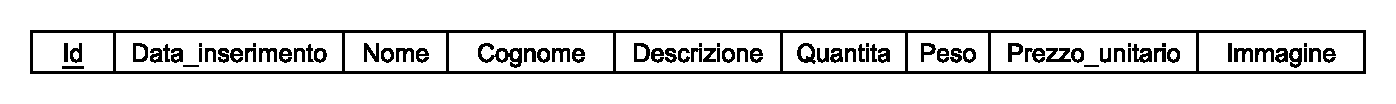
\includegraphics[height=0.04\textheight]{immagini/traduzione_prodotto}

UTENTE\_AMMINISTRATORE\\
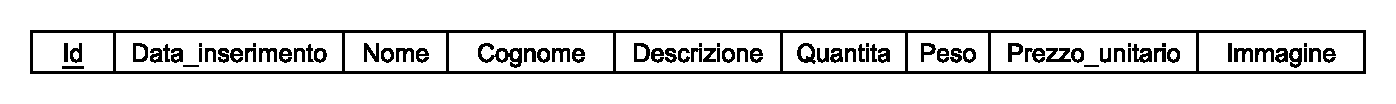
\includegraphics[height=0.04\textheight]{immagini/traduzione_prodotto}
	
UTENTE\_REGISTRATO\\		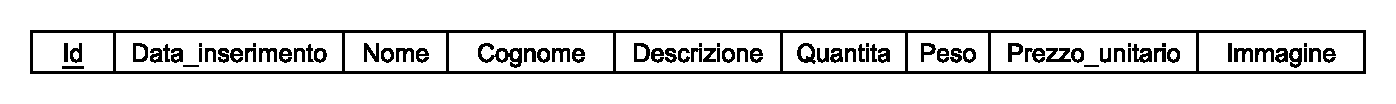
\includegraphics[height=0.04\textheight]{immagini/traduzione_prodotto}

ORDINE\\
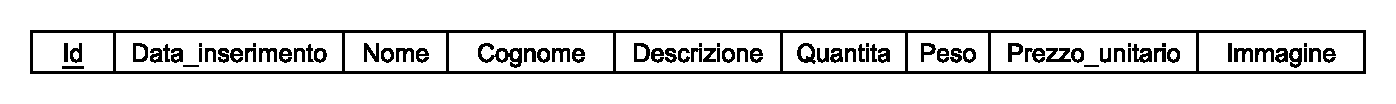
\includegraphics[height=0.04\textheight]{immagini/traduzione_prodotto}
		
PAGAMENTO\\
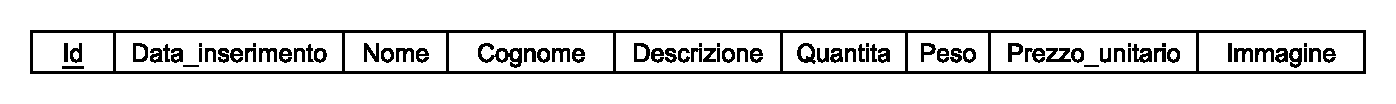
\includegraphics[height=0.04\textheight]{immagini/traduzione_prodotto}
	
FATTURA\\
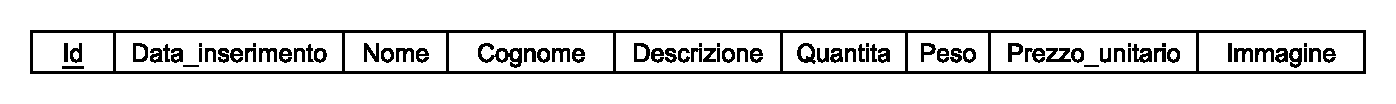
\includegraphics[height=0.04\textheight]{immagini/traduzione_prodotto}
		
RICETTA\\
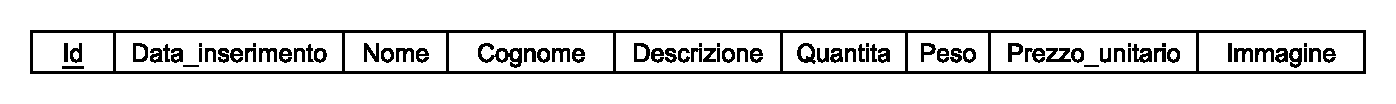
\includegraphics[height=0.04\textheight]{immagini/traduzione_prodotto}
		
MARCHIO\\
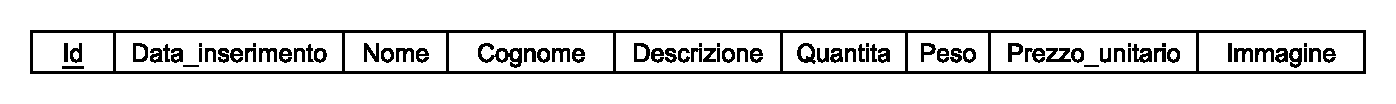
\includegraphics[height=0.04\textheight]{immagini/traduzione_prodotto}
		
CARATTERISTICA\\
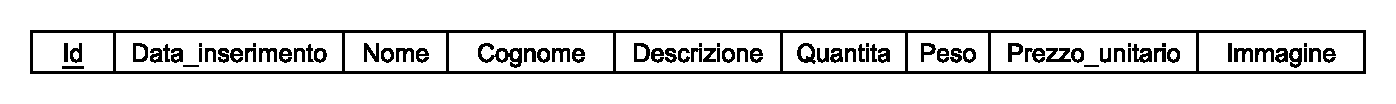
\includegraphics[height=0.04\textheight]
{immagini/traduzione_prodotto}
		
REPARTO\\
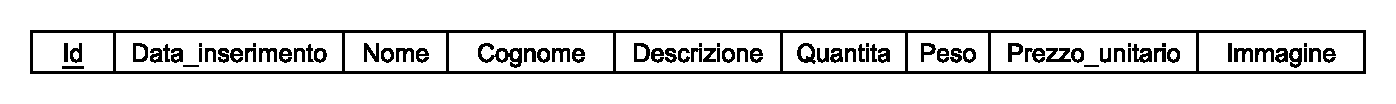
\includegraphics[height=0.04\textheight]
{immagini/traduzione_prodotto}

COUPON\\
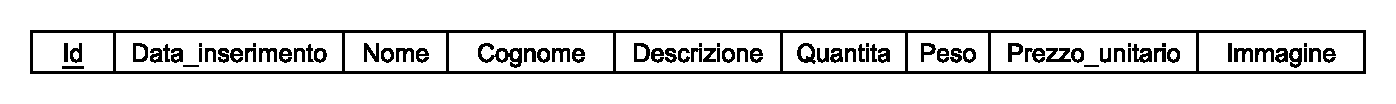
\includegraphics[height=0.04\textheight]{immagini/traduzione_prodotto}

\section{Traduzione di entità deboli}

\section{Traduzione di associazioni binarie 1:1}

\section{Traduzione di associazioni binarie 1:N}

\section{Traduzione di associazioni binarie N:M}